\documentclass[../../header.tex]{subfiles}

\begin{document}

\problem{Three uniform line charges, $\rho_{l1}$, $\rho_{l2}$, and $\rho_{l3}$, each of length $L$, form an equilateral triangle. Assuming that $\rho_{l1}=2\rho_{l2}=2\rho_{l3}$, determine the electric field intensity at the center of the triangle.}

\solution{Aligning the triangle as below, we can tell by symmetry that there will only be an electric field in the $y$ direction.\\
\begin{center}
	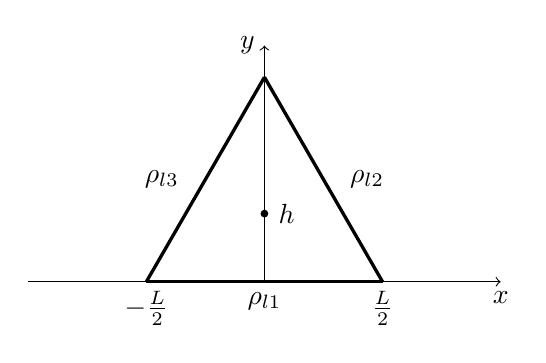
\begin{tikzpicture}[scale=1.5]
		\draw [->] (2,0) -- (2,2) node [left] {$y$};
		\draw [->] (0,0) -- (4,0) node [below] {$x$};
		\draw [very thick] (1,0) -- (3,0) node [midway,below] {$\rho_{l1}$};
		\draw [very thick] (3,0) -- (2,1.732) node [midway,right=0.2cm] {$\rho_{l2}$};
		\draw [very thick] (2,1.732) -- (1,0) node [midway,left=0.2cm] {$\rho_{l3}$};
		\node [below] at (1,0) {$-\frac{L}{2}$};
		\node [below] at (3,0) {$\frac{L}{2}$};
		\node [circle,fill,inner sep=1pt,label=right:$h$] at (2,0.577) {};
	\end{tikzpicture}
\end{center}
The electric field contribution due to each line can be found by integrating over the given line
\begin{align*}
	\vect{E}_{y,1}&=\frac{1}{4\pi\epsilon_0}\int_{-L/2}^{L/2}\frac{\rho_{l1}}{h^2+l^2}\frac{h}{\sqrt{h^2+l^2}}dl\vect{a}_y\\
	&=\frac{\rho_{l1}}{4\pi\epsilon_0}\frac{L}{h\sqrt{h^2+L^2/4}}\vect{a}_y\\
	\vect{E}_{y,2}&=\frac{1}{4\pi\epsilon_0}\int_{-L/2}^{L/2}\frac{\rho_{l2}}{h^2+l^2}\frac{h}{\sqrt{h^2+l^2}}dl\vect{a}_y\left(-\cos{\frac{\pi}{3}}\right)\\
	&=-\frac{\rho_{l2}}{8\pi\epsilon_0}\frac{L}{h\sqrt{h^2+L^2/4}}\vect{a}_y\\
	\vect{E}_{y,3}&=\frac{1}{4\pi\epsilon_0}\int_{-L/2}^{L/2}\frac{\rho_{l3}}{h^2+l^2}\frac{h}{\sqrt{h^2+l^2}}dl\vect{a}_y\left(-\cos{\frac{\pi}{3}}\right)\\
	&=-\frac{\rho_{l3}}{8\pi\epsilon_0}\frac{L}{h\sqrt{h^2+L^2/4}}\vect{a}_y\\
\end{align*}
Using $\rho_{l1}=2\rho_{l2}=2\rho_{l3}$ and the centre of the triangle is at $h=L/2\sqrt{3}$, this simplifies to
\begin{align*}
	\vect{E}=\vect{E}_{y,1}+\vect{E}_{y,2}+\vect{E}_{y,3}=\frac{3\rho_{l1}}{4\pi\epsilon_0L}\vect{a}_y=\frac{3\rho_{l2}}{2\pi\epsilon_0L}\vect{a}_y\\
\end{align*}}
\answer{
\begin{align*}
{\vect{E}=\frac{3\rho_{l2}}{2\pi\epsilon_0L}\vect{a}_y
}
\end{align*}}
\end{document}




































